% don't remove the folling lines, and edit the defintion of \main if needed
\documentclass[../report.tex]{subfiles}
\providecommand{\main}{..}
\IfEq{\jobname}{\currfilebase}{\AtEndDocument{\biblio}}{}
% until here

\begin{document}
\linenumbers
% this is the extra information to be used for the general sections.


%\section{Introduction and Key questions}

From the early observation of a supernova by Tycho Brahe in 1572 to the recent observation in 2017 of a neutron star merger with both gravitational waves and electromagnetic waves ranging from $\gamma$ rays to infrared, the cosmos has always been a rich source of unexpected phenomena and wide-ranging discoveries. Some of these had a deep impact on our understanding of the physical world and its fundamental laws.

This is also true in the realm of particle physics, where many new particles were discovered with cosmic rays. Neutrino oscillations are a case in point, as their study was motivated for a long time by the puzzles posed by solar and atmospheric neutrinos. Cosmic rays are accelerated to energies far beyond the reach of present and future accelerators by processes that are still largely unknown. They offer therefore the possibility to test particle physics in an otherwise inaccessible domain, both in terms of energies and of cosmological propagation distances.

\begin{figure} [htbp!]
\begin{center}
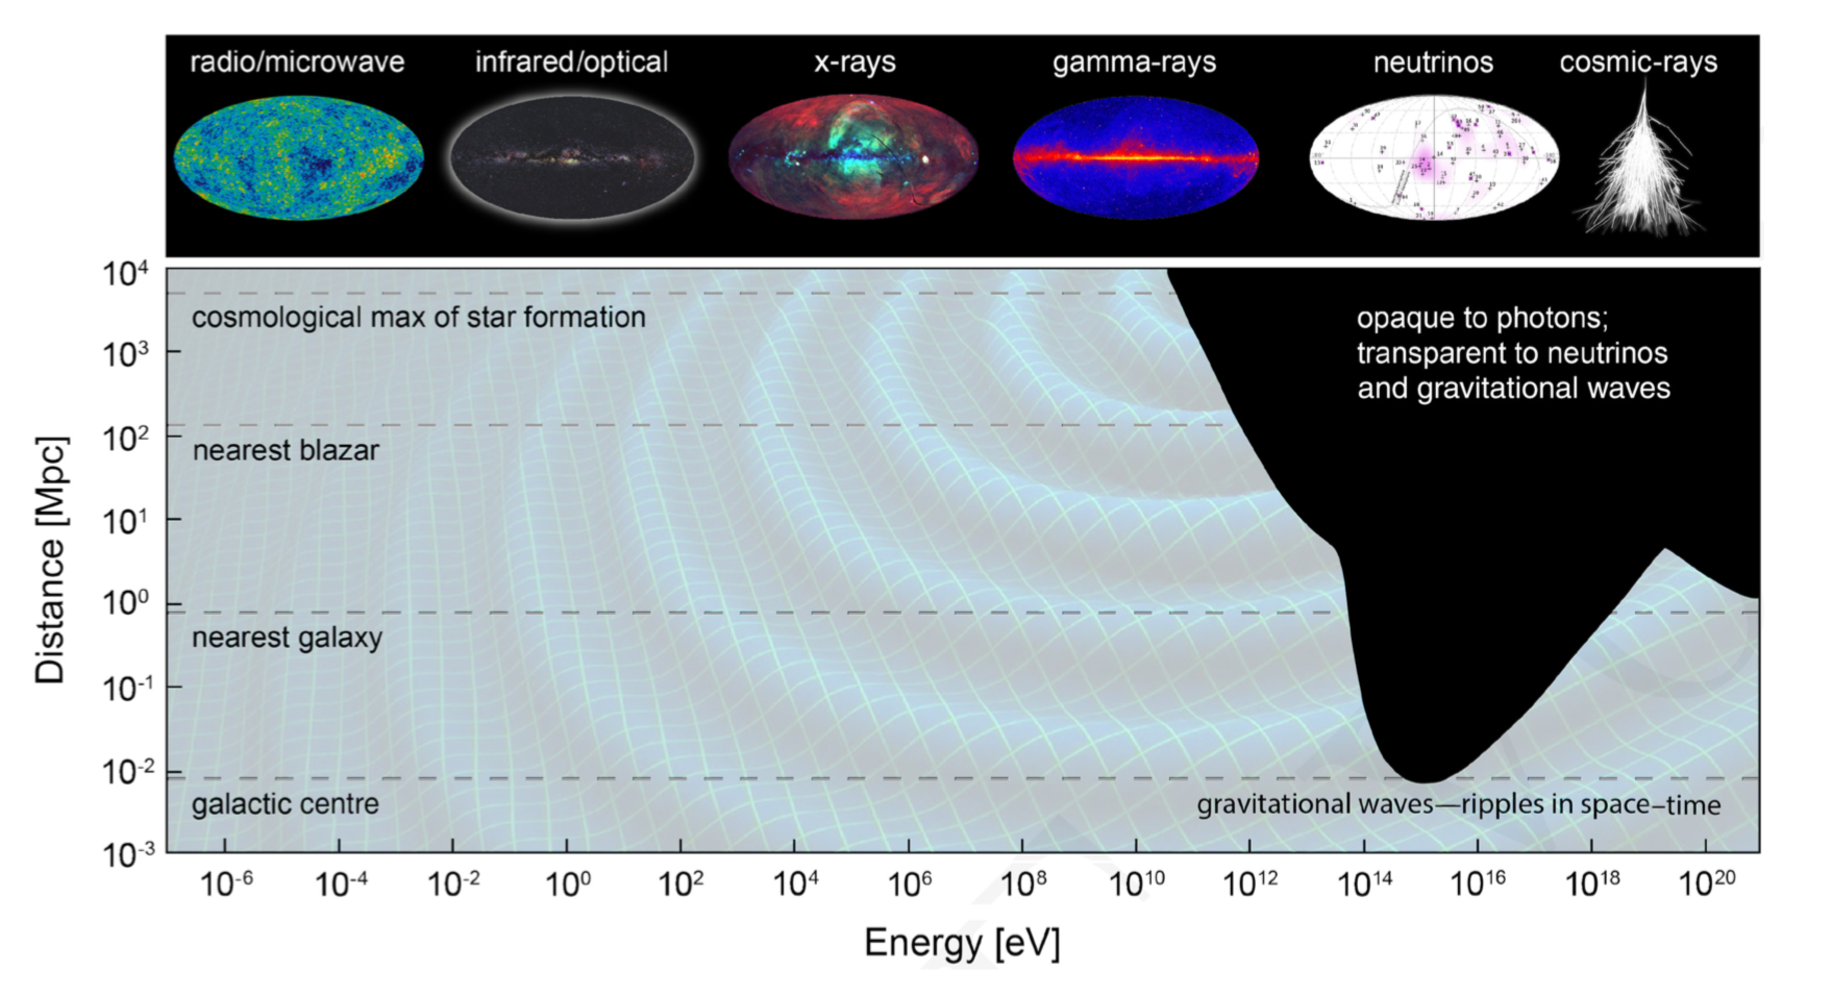
\includegraphics[scale=0.45]{\main/Cosmic/img/multimessenger.pdf}
\caption{\label{fig:multimessenger} Distance horizon at which the Universe becomes optically thick to electromagnetic radiation.% While lower-energy photons can travel to us from the farthest corners of the Universe, the highest energy photons and cosmic rays are attenuated after short distances, obscuring our view of the most energetic cosmic events. 
In contrast, the Universe is transparent to gravitational waves and neutrinos, making them suitable probes of the high-energy sky.
}
\end{center}
\end{figure}
Today many new observatories are in operation or in construction (to name a few: Auger, CTA, IceCube, KM3NeT, ET) and they provide much increased sensitivity, thereby opening up a new domain. This is particularly true for gravitational waves and neutrinos which represent a truly new way of exploring the Universe. Indeed, while lower-energy photons can travel to us from the farthest corners of the Universe, the highest energy photons and cosmic rays are attenuated after short distances, obscuring our view of the most energetic cosmic events. In contrast, the Universe is transparent to gravitational waves and neutrinos, making them suitable probes of the high-energy sky (Fig.~\ref{fig:multimessenger}).
Moreover the simultaneous observation of cosmic events with multiple messengers 
provide new insights in the astrophysical properties of compact objects but also stringent tests of physical laws and particle properties.

In this chapter we will briefly review the various fields and the  observatories
most relevant for this strategy update, before concluding with some considerations on the synergy with particle physics. The European road map for this field has been discussed and prepared by APPEC~[ID84].

\section{Ultra High Energy charged particles} 
\subfile{\main/Cosmic/sub1/UHECR}
\section{Ultra High Energy neutrinos} 
\subfile{\main/Cosmic/sub1/UHEnu}
\subfile{\main/Cosmic/sub1/gwave}
\subfile{\main/Cosmic/sub1/multimessenger}
\subfile{\main/Cosmic/sub1/synergy}
%\section{Relation to other chapters}
%\subsection{Temporary repository for synergy suggestions}
%\subsection{Temporary repository for cross references to be made with other sections}
\end{document}